\chapter{Resolved atomization simulations of BIMER}
\label{ch8:bimer_resolved_atomization}


\section{Introduction}

The multipoint burner BIMER was introduced in Chapter \ref{ch7:bimer_test_bench_and_aero}, where a study of the aerodynamic flow field for the operating conditions of interest was performed. Two operating points were simulated: the one tested by \citeColor[providakis_etude_2013] for which experimental data on the aerodynamic field was available, which was used for validating the simulations performed with YALES2; and the one tested by \citeColor[renaud_high-speed_2015] which provides experimental data on the non-reactive spray state. 

In this chapter, resolved simulations of the atomization process through one injector of the BIMER take-off stage, as done in Chapter \ref{ch5:jicf_resolved_simulations} for the academic JICF test case, are performed. The numerical setup and liquid injection operating point are described in $\S$\ref{sec:ch8_BIMER_computational_setup} and $\S$\ref{sec:ch8_BIMER_operating_condition} respectively. Then, the inlet velocity profiles from the aerodynamic computations which are relevant for jet breakup and droplet transport are shown in $\S$\ref{sec:ch8_BIMER_initial_conditions}. Results from resolved atomization simulations performed for \textbf{XX} interface mesh resolutions are shown in $\S$\textbf{XX}. Finally, injectors learnt and built from such simulations are discussed in $\S$\ref{sec:ch8_learning_SLI_in_BIMER}. These injectors are later used to initialise spray simulations at BIMER in Chapter \ref{ch9:BIMER_lagrangian}.



\section{Computational setup}
\label{sec:ch8_BIMER_computational_setup}

The computational geometry for performing the resolved atomization simulations is the same one as the one used for the aerodynamic ones, displayed in Figure \ref{fig:BIMER_geometry_full_domain}. The fine mesh from Figure \ref{fig:BIMER_mesh_fine} is used, its details provided in Table \ref{tab:BIMER_meshes_gaseous}. The aerodynamic field described in $\S$\ref{ch7:BIMER_application_point} is used as initial condition for the resolved atomization simulations. The boundary conditions are also the same ones in all the boundary except for the liquid injection point, which for the aerodynamic simulations it was specified as solid wall and for the resolved ones is changed to inlet. 

The location of the liquid injection point in the take-off stage is shown in Figure \ref{fig:BIMER_geometry_flower_details}. The injector consists of a nozzle with 8 mm length and a circular cross-section of diameter 0.3 mm. The injection nozzle can be appreciated in Figure \ref{fig:BIMER_liquid_injector_views}, where zoomed-in views of the liquid injection point rear and front sides are shown. The direction of the incoming air $u_g$ and the liquid injection $u_l$ are detailed, as well as the crossflow direction $x_c$ obtained from the resolved atomization simulations (see $\S$\ref{sec:ch8_BIMER_initial_conditions}). A cut of the mesh in the injector is appreciated in the left figure: the cell size within the injector has been set to $35 \sim \mu$m, and the walls are refined to $15 \sim \mu$m. The right figure shows the dimensions of the gaseous inlet channel, which yield a hydraulic diameter of $D_h = 7.5$ mm. 


\begin{figure}[h!]
	\centering
	\includeinkscape[inkscapelatex=false,scale=0.2]{./part3_applications/figures_ch8_resolved/geometry_BIMER_liquid_injector_view/BIMER_liquid_injector_views_2}
	\caption[View of liquid injection point in BIMER]{View of liquid injection point in BIMER. The central figure shows the multipoint injector previously displayed in Figure \ref{fig:BIMER_geometry_flower_details}. The rectangular section shows zoomed-in views of the rear (\textsl{left}) and front (\textsl{right}) sides of the liquid injection point. The rear side shows the nozzle where the liquid inlet boundary condition is applied, and a view of the mesh within the injector. The front side (with transparency in the walls) the injection point where liquid is injected at velocity $u_l$, the crossflow direction $x_c$, and the gaseous inlet channel between two vanes of size 6 x 10 mm$^2$ where enters at a bulk velocity $u_g$.}%{View of liquid injection point in BIMER. The right top figure shows the injection nozzle. A zoomed view of the rectangular section is shown in the right bottom display, where a cut of mesh inside the injector is observed.}
	\label{fig:BIMER_liquid_injector_views}
\end{figure}

\subsubsection*{Sampling planes in BIMER}

The purpose of the BIMER resolved simulations is to characterize the produced spray in order to create lagrangian injectors with the SLI methodology to initialize dispersed phase computations. Therefore, the spray must be sampled in the fashion as it was done for the DLR JICF, whose sampling planes were shown in Figure \ref{fig:jicf_interior_boundaries_surface_measurements}. In that test case, the defined sampling planes were perpendicular to the crossflow axis $x$, since the jet deviates and atomizes producing a spray that moves in this direction. BIMER presents a more complex geometry representative of real injection systems where the absolute reference system is not aligned with the liquid fuel injection point chosen. Therefore, it is convenient to change the reference system to a local one which is aligned with the jet deviation direction (i.e. the local crossflow direction). This direction is denoted as $x_c$ and is shown in Figure \ref{fig:BIMER_liquid_injector_views} right. It has been obtained by performing resolved simulations and checking visually the JICF direction. The local reference system is defined by the orthogonal coordinates $\textbf{x}_c^T =\left\lbrace x_c, y_c, z_c \right\rbrace$ obtained through a transformation from the global coordinate system. This local system, shown in Figure \ref{fig:BIMER_local_FoR_and_sampling_planes}, is centered at the liquid injection point. The figure also shows the location of the sampling planes, which are perpendicular to the $x_c$ axis and are expressed in relation to the injection diameter $d_\mathrm{inj}$. In all simulations performed, a sponge layer where liquid is artificially suppressed has been located at $x_c/d_\mathrm{inj} = 12$ to reduce the cost of the computations.

\begin{figure}[h!]
	\centering
	\includeinkscape[inkscapelatex=true,scale=0.8]{./part3_applications/figures_ch8_resolved/BIMER_local_FoR_and_sampling_planes}
	\vspace*{-0.5in}
	\caption{Instaneous snapshot of liquid injection in BIMER shown the local coordinate system and the location of spray sampling planes. \textbf{XX OJO: actualizar con sampling planes finales.}}
	\label{fig:BIMER_local_FoR_and_sampling_planes}
\end{figure}


\section{Operating condition}
\label{sec:ch8_BIMER_operating_condition}

The ambient conditions and inlet gaseous flow rate for the operating point to study are shown in Table \ref{tab:gaseous_operating_points_BIMER}. These ones characterize the aerodynamic field of the overall burner. To determine now the operating point and classify it into the JICF breakup map, the liquid and gaseous parameters relevant to the single multipoint injector need to be stated.

%\begin{equation}
%x/d_\mathrm{inj} ~~ ; ~~ \textcolor{blue}{z/d_\mathrm{inj} }
%\end{equation}

\subsubsection*{Gaseous phase}

%According to \citeColor[barbosa_etude_2008], $80 \%$ of the air flow rate goes through the take-off stage and $20 \%$ goes through the take-off one. The study of \citeColor[renaud_high-speed_2015] shows that the percentage through the pilot is actually $13.5 \%$, hence $86.5 \%$ goes through the take-off. Considering the application point in Table \ref{tab:gaseous_operating_points_BIMER}, this makes a total of $\dot{m}_{g,\mathrm{takeoff}} = 37.2815 ~ $ g s$^{-1}$, which corresponds to a flow rate $Q = 0.04567 $ m$^{3}$ s$^{-1}$. Since that this flow rate is split through 20 vanes, the flow rate per canal is $Q_g = 2.2833 \cdot 10^{-3}$ m$^{3}$ s$^{-1}$. With an area of 6x10 mm$^2$ (see Figure \ref{fig:BIMER_liquid_injector_views}), the estimated gas bulk velocity is:

%\begin{equation}
%u_g = Q_g/A = 38 ~ \mathrm{m} ~ \mathrm{s}^{-1}
%\end{equation}

The aerodynamic field inside BIMER for the operating points of interest was discussed in Chapter \ref{ch7:bimer_test_bench_and_aero}. From this study, a fine mesh consisting of 38 million elements was chosen (see Table \ref{tab:BIMER_meshes_gaseous}). The gaseous field for the application point, which is the chosen one to perform spray simulations, was studied in $\S$\ref{ch7:BIMER_application_point}. This solution is taken as the initial condition from the resolved atomization simulations.

For the resolved atomization simulations, the relevant gas conditions are those found close to the liquid injection point. In the case of a simple JICF geometry like the one studied in Chapter \ref{ch5:jicf_resolved_simulations}, the gas and liquid flows directions are known, and the gaseous conditions impinging the jet and relevant for liquid breakup are easily determined. For a complex geometry, swirled injector such as BIMER, the crossflow direction is not known a prior and needs to be determined. For such purpose, resolved simulations are a useful tool since they provide all the information regarding the jet. For determining the crossflow reference system $\textbf{x}_c$, displayed in Figure \ref{fig:BIMER_local_FoR_and_sampling_planes},  a first simulation was run and the direction in which droplets were convected was taken as the crossflow direction $x_c$. 

Figure \ref{fig:BIMER_Umean_profile_with_jet} left shows the gas mean streamlines through the inlet vane of the multipoint stage that impinge the crossflow. An instantaneous view of the jet is shown for visualization, although the streamlines correspond to the gaseous solution without the jet. As observed, the jet is fully immersed within the gas coming through the closest vane, and is not affected by the gas coming from the neighbouring vanes. The streamlines also show a high variation in the velocity magnitude along the vane width, with the highest velocity streamlines being the ones affecting the jet. The jet crossflow direction $x_c$ is also indicated in the view. Figure \ref{fig:BIMER_Umean_profile_with_jet} right shows the mean axial velocity field in the middle crossflow plane $y_c = 0$. The velocity coordinates have been transformed from the absolute coordinate system to the crossflow one, hence the axial velocity displayed $\overline{u}_c$ is the one in the crossflow direction. The arrows show the velocity profile along the crossflow vertical direction $z_c$ at a location $x_c/d_\mathrm{inj} = -0.5$, i.e. right upstream the injector (it has been shifted in the figure to allow for visual comparison with the jet). This profile, together with the $TKE$ profile along the same line, are plotted in Figure \ref{fig:BIMER_gas_inlet_profiles}. A bulk gaseous velocity $u_g = 56 ~\mathrm{m}.\mathrm{s}^{-1}$ is obtained as the mean of the gaseous velocity profile. The TKE profile shows high values in general along all the vertical coordinate, which reflects a high turbulent state of the flow created by the swirled injector. %From the walls upwards, the $TKE$ firstly increases and then undergoes a decrease at $x_c \sim 1$ to then start augmenting again at the center of the channel. 


\begin{figure}[ht]
\centering
\includegraphics[scale=0.225]{./part3_applications/figures_ch8_resolved/gaseous_profile_streamlines_and_vector}
\caption[Gaseous state at the vicinity of the liquid injection location]{Gaseous state at the vicinity of the liquid injection location. \textsl{Left}: gas streamlines through the inlet multipoint vane.  \textsl{Right}: Instaneous BIMER view with mean axial velocity field in plane $y_c = 0$. The mean field corresponds to the gaseous solution without liquid used as an inlet condition, the jet has been added for comparison. The vectors represent the velocity profile just upstream the injector. The velocity profile has been displaced upstream in the picture for a better visualization.}
% OJO: ficheros generados para el perfil de velocidades estan en Ongoing\ICS_study\u_mean_profiles\cases_probes\mesh_refined_DX0p5_ics_no_actuator_flat_BL_with_turbulence_L3p00_up2p7
\label{fig:BIMER_Umean_profile_with_jet}
\end{figure}



\begin{figure}[ht]
\centering
	\centering
   \includegraphics[scale=0.4]{./part3_applications/figures_ch8_resolved/gas_inlet_profiles}
   \vspace*{-0.15in}
   \caption{Profiles of $\overline{u}_c$ and $TKE$ along the vertical line right upstream the liquid injector}
\label{fig:BIMER_gas_inlet_profiles}
\end{figure}




\subsubsection*{Liquid phase}

In the operating point studied, the total liquid mass flow rate injected is $\dot{m}_{l,\mathrm{total}} = 1.64$ g s$^{-1}$. The staging parameter, defined in Eq. (\ref{eq:BIMER_staging_parameter}), is $\alpha = 15 ~\%$, meaning that amount of liquid goes through the pilot stage and $85 ~\%$ of fuel goes through the take-off. Therefore, $\dot{m}_{l,\mathrm{pilot}} = 0.25$ g s$^{-1}$ and $\dot{m}_{l,\mathrm{takeoff}} = 1.39$ g s$^{-1}$. This quantity of fuel is injected through 10 injection holes that conform the take-off stage; assuming that fuel repartition is done equally through all the channels, each injector introduces $0.139$ g s$^{-1}$ of dodecane fuel, which is equivalent to a flow rate of $Q_l = 185.3$  mm$^3$ s$^{-1}$ given the dodecane density from Table \ref{tab:dodecane_properties}. From this flow rate, the bulk liquid velocity $u_l$ can be estimated knowing an injection diameter of $d_\mathrm{inj} = 0.3$ mm:

\begin{equation}
u_l = \frac{Q_l}{\pi d_\mathrm{inj}^2 / 4} = 2.6 ~ \mathrm{m}.\mathrm{s}^{-1}
\end{equation}


The velocity profile imposed at the liquid inlet shown in Figure \ref{fig:BIMER_liquid_injector_views} is a Poiseuille profile with the mean velocity of value $u_l$. With the estimate values for bulk liquid and gaseous velocities, the liquid properties given in Table \ref{tab:dodecane_properties} and the gaseous properties from Table \ref{tab:gaseous_operating_points_BIMER}, the momentum flux ratio $q$ and the Weber number based on the gaseous phase $We_g$ can now be calculated:

%\begin{subequations}
%\begin{align}
%q &=  \frac{\rho_l u_l^2}{\rho_g u_g^2} \approx 4 \\
%We_g &=  \frac{\rho_g d_{inj} u_g^2}{\sigma} \approx 14
%\end{align}
%\end{subequations}

\begin{equation}
q =  \frac{\rho_l u_l^2}{\rho_g u_g^2} \approx 2 ~~~~ ; ~~~~  We_g =  \frac{\rho_g d_\mathrm{inj} u_g^2}{\sigma} \approx 30
\end{equation}

%\begin{subequations}
%\begin{align}
%q &=  \frac{\rho_l u_l^2}{\rho_g u_g^2} = \frac{750 \cdot 2.6^2}{0.816382 \cdot 38.05^2} = 4 \\
%We_g &=  \frac{\rho_g d_{inj} u_g^2}{\sigma} = \frac{0.816382 \cdot 0.3 mm \cdot 38.05^2}{25.35 10^{-3}} \approx 14
%\end{align}
%\end{subequations}

Figure \ref{fig:location_BIMER_op_in_breakup_map} shows the BIMER JICF operating point classified in the breakup diagram of \citeColor[wu_breakup_1997], which is located within the multimode breakup regime. The governing parameters characterizing the BIMER operating point are summarized in Table \ref{tab:bimer_sps_operating_point}. The dimensionless numbers from Eqs. (\ref{eq:dimensionless_numbers_jicf}) are also calculated. \hl{\textbf{XX:}Three} simulations have been performed with three different element resolutions at the liquid-gas interface $\Delta x_\mathrm{min}$, the nomenclature for each case is given in Table \ref{tab:BIMER_resolved_simulations_performed}.

\begin{figure}[ht]
     \centering
     \includeinkscape[inkscapelatex=false,scale=0.6]{./part3_applications/figures_ch8_resolved/BIMER_breakup_regime_our_operating_point}
     \vspace*{-0.1in}
     \caption{Location of simulated operating condition in the breakup map by \citeColor[wu_breakup_1997]}
	% See: https://stackoverflow.com/questions/35210337/can-i-plot-several-histograms-in-3d/35225919
      \label{fig:location_BIMER_op_in_breakup_map}
\end{figure}

\begin{table}[!h]
\centering
\caption{BIMER operating point to perform resolved atomization simulations}
\begin{tabular}{lccc}
\thickhline
\textbf{Parameter} & \textbf{Symbol} & \textbf{Units} &  \textbf{Value} \\
\thickhline
Nozzle diameter & $d_\mathrm{inj}$ & mm & 0.3 \\
%\hline
Gas bulk velocity & $u_g$ & m s$^{-1}$ & 56 \\
%\hline
Gas flow rate & $Q_g$ & m$^3$ s$^{-1}$ & $2.2833 \cdot 10^{-3}$   \\
%\hline
Liquid bulk velocity & $u_l$ & m s$^{-1}$ & 2.6  \\
%\hline
Liquid flow rate & $Q_l$ & mm$^3$ s$^{-1}$ & 185.3  \\
%\hline
Ambient pressure & $p_\mathrm{amb}$ & bar &  1 \\
%\hline
Gas temperature & $T_g$ & K & 433 \\
%\hline
Liquid temperature & $T_l$ & K &  \\
%\hline
Gas density & $\rho_g$ & kg m$^{-3}$ & 0.82 \\
%\hline
Liquid density & $\rho_l$ & kg m$^{-3}$ & 750 \\
%\hline
Gas viscosity & $\mu_g$ & kg m$^{-1}$ s$^{-1}$ & $2.39 \cdot 10^{-5}$ \\
%\hline
Liquid viscosity & $\mu_l$ & kg m$^{-1}$ s$^{-1}$ &  $1.36 \cdot 10^{-3}$ \\
%\hline
Surface tension & $\sigma$ & kg s$^{-2}$ &  0.025  \\
\thickhline
Gas Reynolds number & $Re_g$ & - & $20 \cdot 10^3$ \\ %& $9.80 \cdot 10^3$ \\
%\hline
Liquid Reynolds number & $Re_l$ & - & 430 \\
%\hline
Momentum ratio & $q$ & - & 1 \\ %4  \\
%\hline
Gas Weber number & $We_g$ & - & 55 \\ %14 \\
%\hline
Liquid Weber number & $We_l$ & - & 60 \\
%\hline
Relative Weber number & $We_\mathrm{rel}$ & - & 52 \\ %12 \\
%\hline
Aerodynamic Weber number & $We_\mathrm{aero}$ & - & 0.067 \\
%\hline
Ohnesorge number & $Oh $ & - & 0.018 \\
%\hline
Density ratio & $r$ & - & 915 \\
%\hline
\thickhline
\end{tabular}
\label{tab:bimer_sps_operating_point}
\end{table}

\begin{table}[!h]
\centering
\caption{Nomenclature for resolved atomization simulations}
\begin{tabular}{cc}
\thickhline
%$\pmb{\Delta} x_\mathrm{min}$ [$\pmb{\mu}$$\textbf{m}])  &  \multicolumn{2}{c}{\textbf{Operating condition}} \\ 
$\Delta x_\mathrm{min}$ [$\mu$m]  &  Denomination \\ 
\thickhline
7.5 & BIMER\_DX07 \\
10 & BIMER\_DX10 \\
15 & BIMER\_DX15 \\
\thickhline
\end{tabular}
\label{tab:BIMER_resolved_simulations_performed}
\end{table}




\section{Definition of liquid characteristic times}

Characteristic times can be defined for the liquid phase in BIMER in the same way it was done for the DLR JICF test case from Chapter \ref{ch5:jicf_resolved_simulations}. Details on the timescales chosen and on their calculation are given in $\S$\ref{sec:ch5_liquid_characteristic_times}. Here, the definitions summarized in Table \ref{tab:jicf_characteristic times} are directly applied to the BIMER test case. The results are shown in Table \ref{tab:BIMER_SPS_characteristic times}. 

\begin{table}[!h]
\centering
\caption{Characteristic physical timescales [$\mu$s] in BIMER simulations}
\begin{tabular}{ccc}
\thickhline
\textbf{Time scale} & \textbf{Expression} & \textbf{BIMER} \\
\thickhline
Inertia & $\tau_\mathrm{in} = \frac{d_\mathrm{inj}}{u_l}$ & 115.38 \\
Aerodynamic breakup  &  $\tau_\mathrm{ab} =  \frac{d_\mathrm{inj}}{u_g - u_l} \sqrt{\frac{\rho_l}{\rho_g}} $ & 256.30 \\
Non-aerodynamic breakup  &  $\tau_\mathrm{nb} = \frac{d_\mathrm{inj}}{u_l} We_l^{1/3} $ &  453.81 \\
Capillary & $\tau_\mathrm{cap} = \sqrt{\frac{\rho_l d_\mathrm{inj}^3}{8 \sigma}}$ & 318.20 \\
\thickhline
\end{tabular}
\label{tab:BIMER_SPS_characteristic times}
\end{table} 

As shown in the previous table, the lower timescale is found for the inertia processes and hence those are governing breakup. Yet, all timescales are of the same order of magnitude, as opposed to the timescales of the DLR JICF summarized in Figure \ref{tab:jicf_characteristic times} where the fastest timescale (inertia) was around $100$ times smaller than the slowest (capillary). For the BIMER operating point studied, the inertia timescale is only $3$ times smaller than the capillary one, which is not even the slowest (in this case, it corresponds to the non-aerodynamic breakup timescale). The fact that the timescales in this case are closer to each other agree with the location of the BIMER operating point in the breakup diagram of Figure \ref{fig:location_BIMER_op_in_breakup_map} \citepColor[pilch_use_1987]. Besides the physical timescales, the droplets arrival times to the sampling planes depicted in Figure \ref{fig:BIMER_local_FoR_and_sampling_planes}. These ones are summarized in Table \ref{tab:BIMER_SPS_characteristic_droplet_sampling_times}. 


%\begin{table}[!h]
%\centering
%\caption{Characteristic droplet arrival times to sampling planes $\tau_\mathrm{dr_{x_c}}$ [$\mu$s] in BIMER simulations}
%\begin{tabular}{ccccccc}
%\thickhline
%\textbf{Case} & $x_c/d_\mathrm{inj} = 3.33$ & $x_c/d_\mathrm{inj} = 5$ & $x_c/d_\mathrm{inj} = 6.67$ & $x_c/d_\mathrm{inj} = 8.33$ & $x_c/d_\mathrm{inj} = 10$ & $x_c/d_\mathrm{inj} = 11.66$  \\
%\thickhline 
%BIMER\_DX07 & 321 & 340 & 359 & 395 & 434 & 589 \\
%BIMER\_DX10 & 310 & 331 & 354 & 387 & 428 & 585 \\
%BIMER\_DX15 & 450 & 511 & 562 & 569 & 633 & 729 \\
%\thickhline
%% NOTA: valores DX07 corresponden en realidad a dx_min = 5 µm
%% NOTA: valores DX07 a partir de 8.33 han sido estimados a ojo
%\end{tabular}
%\label{tab:BIMER_SPS_characteristic_droplet_sampling_times}
%\end{table}


\begin{table}[!h]
\centering
\caption{Characteristic droplet arrival times to sampling planes $\tau_\mathrm{dr_{x_c}}$ [$\mu$s] in BIMER simulations}
\begin{tabular}{cccc}
\thickhline
\textbf{Case} & $x_c/d_\mathrm{inj} = 3.33$ & $x_c/d_\mathrm{inj} = 5$ & $x_c/d_\mathrm{inj} = 6.67$  \\
\thickhline 
BIMER\_DX07 & 321 & 340 & 359 \\
BIMER\_DX10 & 310 & 331 & 354 \\
BIMER\_DX15 & 450 & 511 & 562 \\
\thickhline
% NOTA: valores DX07 corresponden en realidad a dx_min = 5 µm
% NOTA: valores DX07 a partir de 8.33 han sido estimados a ojo
\end{tabular}
\label{tab:BIMER_SPS_characteristic_droplet_sampling_times}
\end{table}




\section{Jet evolution}

The jet evolution at the early instants of the injection process is shown in Figure \ref{fig:BIMER_jet_establishment}. Snapshots are shown for values of dimensionless time $t^*$ defined by Eq. (\ref{eq:t_dimensionless_with_tau_in}), in which the physical time is expressed in relation to the timescale $\tau_\mathrm{in}$ from Table \ref{tab:BIMER_SPS_characteristic times}. As in the simulations from Chapter \ref{ch5:jicf_resolved_simulations}, this timescale has been chosen since is the same for all simulations and the jets depicted represent therefore equivalent instants.

Images show the features of a liquid JICF configuration: the jet leaves the injection nozzle and enters into contact with the crossflow, which has the effect of deforming the liquid column and deviating the jet towards the crossflow direction (which is represented in Figure \ref{fig:BIMER_jet_establishment} by the black solid line). However, the jet topology is very different to a classical JICF configuration such as the one studied in Chapter \ref{ch5:jicf_resolved_simulations}: both surface and column breakup are present (more details are given on the next section), but in BIMER column breakup creates mainly thin liquid sheets that are quickly disintegrated into small droplets (more details are given on the next section). The jet does not penetrate far and the deviation of the jet column towards the crossflow direction is not highly significant, since breakup occurs close to the injection location (as demonstrated in $\S$\ref{ch8:sec_BIMER_DC_characterization}). The low penetration is due to the low value of $q$ for this operating point, which is the parameter governing the jet penetration. The quick disintegration to low droplets and the instabilities shown along the liquid columns, which are clearly different to the column waves alanyzed in $\S$\ref{subsec:ch5_instabilities_presence} for the classical JICF configuration), are attributed to the highly turbulent state of the flow, as shown by the $TKE$ profile in Figure \ref{fig:BIMER_gas_inlet_profiles}.



%\label{ch8:resolved_atomization_simulations}

%\begin{table}[!h]
%\centering
%\caption{Operating point}
%\begin{tabular}{cccc}
%\thickhline
%$u_g$ [m s$^{-1}$] &  38 \\
%\hline
%$u_l$ [m s$^{-1}$] &  2.6 \\
%\hline
%\hline
%$q$ & 4 \\ %4.3 \\
%\hline
%$We_g$ & 14 \\
%\hline
%\end{tabular}
%\label{tab:bimer_sps_operating_point}
%\end{table}
%
%\begin{table}[!h]
%\centering
%\caption{Operating point}
%\begin{tabular}{cccc}
%\thickhline
%$u_g$ [m s$^{-1}$] &  $u_l$ [m s$^{-1}$] & $q$ &  $We_g$  \\
%\hline
%38 &  2.6 & 4 & 15 \\
%\thickhline
%\end{tabular}
%\label{tab:bimer_sps_operating_point}
%\end{table}



%\begin{figure}[h!]	
%	\centering
%	\includeinkscape[inkscapelatex=false,scale=0.75]{./part1_numerical_approaches/figures_ch3/gas_injection_area_multipoint}
%	\caption{Area to calculate bulk gas velocity}
%	\label{fig:gas_injection_area_multipoint}
%\end{figure}


%According to \textbf{2016 Eckel}, the velocity is not the gaseous one but the relative:
%
%\begin{equation}
%\tau_c = \sqrt{\frac{\rho_l}{\rho_g}} \frac{d_\mathrm{inj}}{u_\mathrm{rel}} = \sqrt{\frac{750}{0.816382 }} \frac{0.3 ~mm}{38 - 2.6} = 0.26
%\end{equation}
%
%which is actually very similar.



%\subsection{Breakup topology}

%The topology is super different with respecto to DLR JICF!! 



\clearpage

\begin{figure}[ht]
\centering
\includeinkscape[inkscapelatex=false,scale=0.7]{./part3_applications/figures_ch8_resolved/jet_establishment}
\caption[Establishment of BIMER resolved atomization simulations at several time instants.]{Establishment of BIMER resolved atomization simulations at several time instants. \textsl{Left}: DX07. \textsl{Center}: DX10. \textsl{Right}: DX15. }
\label{fig:BIMER_jet_establishment}
\end{figure}

\clearpage

\subsection{Breakup topology}
\label{ch8:subsec_BIMER_breakup_topology}

\begin{figure}[ht]
\centering
\includegraphics[scale=0.125]{./part3_applications/figures_ch8_resolved/breakup_topology/DX10_breakup_both}
\caption{Breakup in BIMER, case DX10. }
% Soluciones:
% column breakup: sol02_37, sol03_08,_20,_32, sol04_07,_19
% surface breakup:sol03_32,37, sol04_05,10,13
\label{fig:BIMER_breakup_topology}
\end{figure}


\subsection{Jet establishment}

Esbalishment of the liquid jet in the BIMER configuration is monitored by quantifying the evolution of the number of mesh elements and the liquid volume inside the domain calculated from Eq. (\ref{eq:liquid_volume_from_levelset_definition}). Time has been non-dimensionalized with the timescale $\tau_{\mathrm{dr}_{x_c/d_\mathrm{inj}=6.67}}$ as given in Table \ref{tab:BIMER_SPS_characteristic_droplet_sampling_times}:

%\begin{equation}
%\label{eq:t_prime_BIMER_with_tau_drx10}
%t^{\prime} = \frac{t}{\tau_{\mathrm{dr}_{x_c/d_\mathrm{inj}=10}}}
%\end{equation}

\begin{equation}
\label{eq:t_prime_BIMER_with_tau_drx10}
t^{\prime} = t / \tau_{\mathrm{dr}_{x_c/d_\mathrm{inj}=6.67}}
\end{equation}

Results are shown in Figure \ref{fig:BIMER_volume_nelem_evolution}. Volume increase linearly at the early instants of injection due to the constant flow rate observed. At a certain point, the slope of $V_l$ due to droplets being removed from the simulation when reaching the sponge layer. Liquid volume shows establishent for cases DX10, DX15 at a value between $V_l = 0.75$ and $0.8$ mm$^3$, while simulation DX07 has not yet reached establishment in terms of liquid volume. The evolution of the number of elements in the simulation shows a fast establishment for $DX15$ at a value around $60 \cdot 10^6$ elements. Case DX10 shows maximum values around $100 \cdot 10^6$ elements, while case DX07 reaches a peak around $300 \cdot 10^6$ elements: these too cases show still oscillations (simulation DX10 displays also oscillations for $V_l$ at the last time instants) and might still converge to different values if simulations were run for longer. The oscillations are specially notorious for DX07, since a variation from the peak at $300 \cdot 10^6$ elements until the subsequent value close to $200 \cdot 10^6$ elements supposes a variation in $100 \cdot 10^6$ elements, which is one order of magnitude larger than the amplitude of the oscillations for case DX10. Such variations in the evolution of $V_l$ and number of elements are attributed to  clusters of droplets produced by the column breakup phenomenon reaching the liquid suppression location at similar instants: as Figure \hl{\textbf{XX} shows, the column breakup is highly intermitent and ...}

\begin{figure}[ht]
\centering
\begin{subfigure}[b]{0.45\textwidth}
	\centering
   \includegraphics[scale=0.2]{./part3_applications/figures_ch8_resolved/BIMER_liquid_volume_increase}
   %\caption{Liquid volume}
   \label{fig:BIMER_liquid_volume_evolution} 
\end{subfigure}
\hfill
\begin{subfigure}[b]{0.45\textwidth}
	\centering
   \includegraphics[scale=0.24]{./part3_applications/figures_ch8_resolved/BIMER_nelem_increase}
   %\caption{Zoomed-in view of Figure \ref{fig:JICF_nelem_increase_all_t} in range $t^{\prime} \in [0, 2]$}
   \label{fig:BIMER_nelem_increase}
\end{subfigure}
   \caption[Evolution of number of mesh elements (\textsl{left}) and number of mesh elements (\textsl{right}) with time in BIMER resolved simulations]{Evolution of number of mesh elements (\textsl{left}) and number of mesh elements (\textsl{right}) with time in BIMER resolved simulations. The dashed, black vertical line corresponds to $t^\prime = 1$, time instant when the first droplet reaches the sampling plane $x_c/d_\mathrm{inj} = 10$}
\label{fig:BIMER_volume_nelem_evolution}
\end{figure}

\clearpage

\section{Perturbation effect ot jet dense core}
\label{ch8:sec_BIMER_DC_characterization}

\subsection{Dense core topology characterization}

In order to characterize the dense core topology, the methodology detailed in $\S$\ref{subsec:ch5_jet_dense_core_extraction} is applied. The dense core is represented by its breakup point coordinates $\left( x_b, z_b \right)$ and its width $w$.

\begin{figure}[ht]
\flushleft
\begin{subfigure}[b]{0.45\textwidth}
	\centering
   \includegraphics[scale=0.25]{./part3_applications/figures_ch8_resolved/results_dense_core_modeling/instant_xb_zb_w_DX07}
   \vspace*{-0.30in}
   \caption{Case DX07}
   \label{fig:instant_xb_zb_BIMER_w_DX07} 
\end{subfigure}
\hfill
\begin{subfigure}[b]{0.45\textwidth}
	\centering
   \includegraphics[scale=0.25]{./part3_applications/figures_ch8_resolved/results_dense_core_modeling/instant_xb_zb_w_DX10}
   \vspace*{-0.30in}
   \caption{Case DX10}
   \label{fig:instant_xb_zb_BIMER_w_DX10}
\end{subfigure}

\vskip\baselineskip

\begin{subfigure}[b]{0.9\textwidth}
	\centering
   \includegraphics[scale=0.25]{./part3_applications/figures_ch8_resolved/results_dense_core_modeling/instant_xb_zb_w_DX15}
   \vspace*{-0.30in}
   \caption{Case DX15}
   \label{fig:instant_xb_zb_BIMER_w_DX15} 
\end{subfigure}
   \caption{Variation with time of the BIMER dense core breakup point coordinates $x_\mathrm{b}, z_\mathrm{b}$ and width $w$.}

\label{fig:BIMER_xb_zb_w_evolution}
\end{figure}


\begin{figure}[ht]
\flushleft
\begin{subfigure}[b]{0.3\textwidth}
	\flushleft
   \includegraphics[scale=0.225]{./part3_applications/figures_ch8_resolved/results_dense_core_modeling/convergence_mean_xb}
\end{subfigure}
\hfill
\begin{subfigure}[b]{0.3\textwidth}
	\flushleft
   \includegraphics[scale=0.225]{./part3_applications/figures_ch8_resolved/results_dense_core_modeling/convergence_mean_zb}
\end{subfigure}
\hfill
\begin{subfigure}[b]{0.3\textwidth}
	\flushleft
   \includegraphics[scale=0.225]{./part3_applications/figures_ch8_resolved/results_dense_core_modeling/convergence_mean_width}
\end{subfigure}
   \caption{Evolution of mean geometric parameters of BIMER dense core}
\label{fig:BIMER_DC_mean_parameters_convergence}
\end{figure}

\clearpage

\begin{figure}[ht]
\flushleft
\begin{subfigure}[b]{0.45\textwidth}
	\centering
   \includegraphics[scale=0.25]{./part3_applications/figures_ch8_resolved/results_dense_core_modeling/map_xb_zb}
   \label{fig:BIMER_dense_core_mean_parameters_scatterplots_zb_xb}
\end{subfigure}
%\hfill
\hspace{0.25in}
\begin{subfigure}[b]{0.45\textwidth}
	\centering
   \includegraphics[scale=0.25]{./part3_applications/figures_ch8_resolved/results_dense_core_modeling/map_xb_width}
   \label{fig:BIMER_dense_core_mean_parameters_scatterplots_w_xb}
\end{subfigure}
   \vspace*{-0.30in}
\caption{Mean values for the BIMER dense core geometric parameters}
\label{fig:BIMER_DC_mean_parameters_scatterplots}
\end{figure}

\begin{table}[!h]
\centering
\caption{BIMER dense core mean lengths $L_\mathrm{DC}$ and widths $w$ from JICF simulations performed}
\begin{tabular}{cccc}
\thickhline
\textbf{Case} &  DX07 & DX10 & DX15  \\
\hline
$L_\mathrm{DC}/d_\mathrm{inj}$ & 4.66 & 4.83 & 5.44  \\
$w/d_\mathrm{inj}$ & 0.83 & 1.04 & 1.33  \\
\thickhline
\end{tabular}
\label{tab:BIMER_L_DC_values}
\end{table}


\subsection{Force determination in BIMER dense core}


\begin{table}[!h]
\centering
\caption{Pressures and net dense core surfaces in BIMER simulations}
\begin{tabular}{ccccc}
\thickhline
\textbf{Case} & $p_\mathrm{windward}$ [Pa] & $p_\mathrm{leeward}$ [Pa] & $S_\mathrm{DC}$ [mm$^2$]& $|\boldsymbol{F}_\mathrm{DC}|$ [mN] \\
\thickhline 
DX07  & 2340 & 1550 & 0.38 & 0.1 \\
DX10  &  & & 0.44 & \\
DX15 & 2340 & 1550 & 0.57 & 0.3 \\
\thickhline
\end{tabular}
\label{tab:BIMER_dense_core_pressures_and_force_parameters}
\end{table}

\subsection{Turbulent structures in the gaseous field}

Mean axial velocity and flow streamlines in planes perpendicular to the crossflow $x_c/d_\mathrm{inj} =$ \textbf{XX} are shown in Figure \textbf{XX}. Looking at the streamlines, one of the first observations is that the classical CVP pairs typically observed in JICF configurations, visualized in the JICF configuration of DLR in Figure \ref{fig:JICF_turbulent_structures_planes_x}, are not present in BIMER. A possible explanation of missing CVPs in due to the lack of jet deflection towards the axial direction, which was notorious in the classical JICF (see for instance Figure \ref{fig:JICF_establishment_UG100_lateral}) but which is not very pronounced in BIMER, as shown in Figure \ref{fig:BIMER_jet_establishment}. \citeColor[broadwell_structure_1984] argued that the strength of the CVPs is dependent on the momentum transferred to the crossflow by the jet; later, \citeColor[karagozian_analytical_1986] confirmed this statement while also showing that this momentum transfer is not relevant until the jet has been deflected by the crossflow. Since in the present results the BIMER liquid jet does not deflect to a large excent towards the crossflow direction, this hypothesis might explain the absence of CVPs found in the simulations.

\hl{OJO:} para ver vortices en planos iso-x, mirar articulos Denev-Froelich et swirl-jicf-2011.

\begin{figure}[ht]
\flushleft
\begin{subfigure}[b]{0.45\textwidth}
	\centering
   \includegraphics[scale=0.22]{./part3_applications/figures_ch8_resolved/turbulent_structures/line_y0_along_x_zlow}
   %\caption{}
   %\label{} 
\end{subfigure}
\hspace{0.4in}
\begin{subfigure}[b]{0.45\textwidth}
	\centering
   \includegraphics[scale=0.22]{./part3_applications/figures_ch8_resolved/turbulent_structures/line_y0_along_x_zhigh}
   %\caption{}
   %\label{}
\end{subfigure}
\caption{Mean axial velocity evolution along axial coordinate at locations \textbf{XX:??} $z = 1.6, 4$ mm in plane $y = 0$ (lines of Figure \textbf{XX:??})}
\label{fig:BIMER_sps_lines_y0_along_x_ux_mean}
\end{figure}


\begin{figure}[ht]
\centering
   \includegraphics[scale=0.24]{./part3_applications/figures_ch8_resolved/turbulent_structures/lines_y0_along_z_ux_mean}
\caption{Mean axial velocity evolution along vertical coordinate at \textbf{XX:??} $x = 1, 2.5, 5, 10, 15$ mm locations of plane $y = 0$ (lines of Figure \textbf{XX:??})}
\label{fig:BIMER_sps_lines_y0_along_z_ux_mean}
\end{figure}

\clearpage

\section{Direct measurement of liquid fluxes}

Resolved liquid fluxes are obtained in  interior boundaries (IBs) defined at the same location as the sampling planes from Figure \ref{fig:BIMER_local_FoR_and_sampling_planes}. The procedure followed to obtaine these fluxes was described in $\S$\ref{subsec:ch5_interior_boundaries}. Filming planes are not quantified in this case, since these fluxes are not used by the SLI models and it was shown ($\S$\ref{subsec:ch5_mass_conservation_ACLS_set_levelset_band}) that not all the mass losses in the planes perpendicular to the crossflow direction were due to liquid filming, but also to liquid structures reaching a characteristic size of the order of the mesh resolution.

In first place, the instantaneous flux for simulation DX10 are shown in Figure \ref{fig:IB_liquid_flow_rate_inst_evolution_BIMER}. In the same way as in the classical JICF (Figure \ref{fig:IB_liquid_flow_rate_inst_evolution_UG100_DX10}), the instantaneous fluxes show high oscillations around the injected flow rate due to the intermittent behaviour of the JICF: at certain instants there are cluster of droplets produced by the \hl{column breakup mechanism} (\hl{see $\S$}\ref{ch8:subsec_BIMER_breakup_topology}) crossing the sampling planes together, which yield instantaneous flux values larger than the injected $Q_l$ (flux overshoots); while at other instants there are only a few droplets that are convected through those, probably produced by the \hl{surface breakup mechanism} (\hl{see Figure XX}). 




\begin{figure}[ht]
	\centering
   \includegraphics[scale=0.222]{./part3_applications/figures_ch8_resolved/flow_rates_ibs/inst_Q_iso_x_DX10}
   \vspace*{-0.20in}
\caption{Time evolution of instantaneous liquid flow rates $Q_l$ for case DX10}
\label{fig:IB_liquid_flow_rate_inst_evolution_BIMER}
\end{figure}

The evolution of the mean ($\overline{Q}_l$) and RMS ($Q_\mathrm{l,\mathrm{RMS}}$) flow rates through the IBS for all simulations is shown in Figure \ref{fig:IB_mean_RMS_Ql_evolution}. Mean fluxes (Figure \ref{fig:IB_mean_RMS_Ql_evolution}a) show oscillations at the early instants and a later stabilization to converged values. Case DX15 is converged and DX07 is on the verge of convergence. On the contrary, case DX10 shows still oscillations at the last sampling times due to the flux overshoots around $t^\prime \sim 4.2$ shown in Figure \ref{fig:IB_liquid_flow_rate_inst_evolution_BIMER}. Such overshoots are also reflected in the step increase in the RMS signals of Figure \ref{fig:IB_mean_RMS_Ql_evolution}b for the same case. \hl{The coarses case DX15 shows the mean flux at the location $x_c/d_\mathrm{inj} = 0.33$, which is the closest location to the injector, to be larger than the injected mass flow rate: this is due to liquid flow recirculation at this location, since the resolution is coarse and the liquid structures emanating from the dense core stay attached to it... This recirculation has not been observed for the other two resolutions, which indicates that the interface resolution $\Delta x_\mathrm{min} = 15~\mu $m is not enough to resolve BIMER}.

In all simulations, there is a decrease in the mass flux with increasing axial distance $x_c$ as it was also observed in the JICF simulations of Chapter \ref{ch5:jicf_resolved_simulations}. The final mean values of the fluxes, displaed the bar chart of Figure \ref{fig:BIMER_IB_bargraph_mean}, reflect this trend of mass flux reduction in a more visual way. The RMS values are also shown in the same graph by the vertical bars: these ones have large magnitudes, of tthe order of the mass flow rates obtained (see Figure \ref{fig:IB_mean_RMS_Ql_evolution}b), which indicate the high variance in the instantaneous mass flow rates crossing the sampling planes. Even so, the mean fluxes show a good evolution with values close to the injected flow rates, with reductions along the axial distance due to filming and vanishing liquid structures when reaching a size of the order of the mesh resolution, as it was demonstrated in the resolved simualtions of the JICF test case from Chapter \ref{ch5:jicf_resolved_simulations}.

\begin{figure}[ht]
\centering
\begin{subfigure}[b]{0.9\textwidth}
	\centering
   \includegraphics[scale=0.4]{./part3_applications/figures_ch8_resolved/flow_rates_ibs/evolution_mean_Q_iso_x}
   \vspace*{-0.15in}
   \caption{Mean $Q_l$ evolution in IBs perpendicular to crossflow.}
   %\label{} 
\end{subfigure}
\vskip\baselineskip
\begin{subfigure}[b]{0.9\textwidth}
	\centering
   \includegraphics[scale=0.4]{./part3_applications/figures_ch8_resolved/flow_rates_ibs/evolution_RMS_Q_iso_x}
   \vspace*{-0.15in}
   \caption{RMS $Q_l$ evolution in IBs perpendicular to crossflow.}
   %\label{}
\end{subfigure}

\caption{Time evolution of mean and RMS values of $Q_l$ in BIMER IBs}
\label{fig:IB_mean_RMS_Ql_evolution}
\end{figure}



\begin{figure}[ht]
\centering
   \includegraphics[scale=0.3]{./part3_applications/figures_ch8_resolved/flow_rates_ibs/bar_graph_isox_IBs}
\caption{Mean flow rates from IBs perpendicular to crossflow in BIMER}
\label{fig:BIMER_IB_bargraph_mean}
\end{figure}


\clearpage


\section{Spray characterization}

\subsection{Establishment of mean sprays}

\begin{figure}[ht]
	\centering
   \includegraphics[width=0.45\textwidth]{./part3_applications/figures_ch8_resolved/SPRAY_characterization/establishment_and_fluxes/establishment_DX10}
   \includegraphics[width=0.45\textwidth]{./part3_applications/figures_ch8_resolved/SPRAY_characterization/establishment_and_fluxes/establishment_DX15}
   \caption{Establishment of SMD and $Q_l$ in BIMER sprays}
\label{fig:ch8_spray_char_establishment}
\end{figure}



\subsection{Liquid fluxes: lagrangian versus resolved}
\label{subsec:ch8_sli_fluxes_vs_IBs}



\begin{figure}[ht]
	\centering
   \includegraphics[scale=0.25]{./part3_applications/figures_ch8_resolved/SPRAY_characterization/establishment_and_fluxes/fluxes_SLI_vs_IBs}
   \caption{Liquid fluxes provided by interior boundaries (solid color bars) and lagrangian tracking (black-dashed color bars).}
   \label{fig:ch8_fluxes_bargraph_IBs_vs_LGS}
\end{figure}


\subsection{Granulometry}
\label{ch8:subsec_spray_char_granulo}


\begin{figure}[ht]
\centering
   \includegraphics[scale=0.40]{./part3_applications/figures_ch8_resolved/SPRAY_characterization/SMD_values}
   %SMD_values_broken_axis
   \vspace*{-0.2in}
   \caption{Evolution of SMD with axial distance for each simulation.}
   \label{fig:ch8_spray_char_SMD_final}
\end{figure}


%\hl{For the histograms, we can see 2013 Vie.}



\begin{figure}[ht]
\centering
\begin{subfigure}[b]{1.1\textwidth}
	\flushleft
   \includegraphics[scale=0.35]{./part3_applications/figures_ch8_resolved/SPRAY_characterization/histograms_size_volume/DX10_xD05p00_histograms}
   \includegraphics[scale=0.35]{./part3_applications/figures_ch8_resolved/SPRAY_characterization/histograms_size_volume/DX10_xD06p67_histograms}
	\caption{Case DX10}
\end{subfigure}

\vskip\baselineskip

\begin{subfigure}[b]{1.1\textwidth}
	\flushleft
   \includegraphics[scale=0.35]{./part3_applications/figures_ch8_resolved/SPRAY_characterization/histograms_size_volume/DX15_xD05p00_histograms}
   \includegraphics[scale=0.35]{./part3_applications/figures_ch8_resolved/SPRAY_characterization/histograms_size_volume/DX15_xD06p67_histograms}
	\caption{Case DX10}
\end{subfigure}

   \caption{Droplets size ($f_0$) and volume ($f_3$) histograms for all BIMER cases}
\label{fig:ch8_jicf_size_volume_histograms_all}
\end{figure}



\subsection{Liquid velocities}



\begin{figure}[ht]
\flushleft
\begin{subfigure}[b]{1.1\textwidth}
	\flushleft
   \includegraphics[scale=0.25]{./part3_applications/figures_ch8_resolved/SPRAY_characterization/velocities/ux_mean}
   %\hfill
   \includegraphics[scale=0.25]{./part3_applications/figures_ch8_resolved/SPRAY_characterization/velocities/uy_mean}
   %\hfill
   \includegraphics[scale=0.25]{./part3_applications/figures_ch8_resolved/SPRAY_characterization/velocities/uz_mean}
	\caption{Mean velocities in axial, lateral and vertical crossflow directios}
\end{subfigure}

   \caption[Sampled mean liquid velocities for all cases]{Mean liquid velocities for all cases. Solid lines indicate arithmetic average velocities, while dashed ones indicate volume-weighted average velocities.}
\label{fig:ch8_jicf_liquid_mean_velocities_with_x}
\end{figure}

% Volume-weighted velocities: see pilotage 04/06/2021


\begin{figure}[ht]
\centering
\begin{subfigure}[b]{0.3\textwidth}
	\centering
	\hspace*{-0.2in}
   \includegraphics[scale=0.2]{./part2_developments/figures_ch5_resolved_JICF/SPRAY_characterization/velocities/scatterplots_colorbar_z.png}
\end{subfigure}
\begin{subfigure}[b]{0.3\textwidth}
	\centering
	\hspace*{0.36in}
   \includegraphics[scale=0.2]{./part2_developments/figures_ch5_resolved_JICF/SPRAY_characterization/velocities/scatterplots_colorbar_y.png}
\end{subfigure}
\begin{subfigure}[b]{0.3\textwidth}
	\centering
	\hspace*{0.7in}
   \includegraphics[scale=0.2]{./part2_developments/figures_ch5_resolved_JICF/SPRAY_characterization/velocities/scatterplots_colorbar_z.png}
\end{subfigure}

   \vskip\baselineskip
   
   \vspace*{-0.2in}
\begin{subfigure}[b]{0.3\textwidth}
	\flushleft
   \includegraphics[scale=0.2]{./part2_developments/figures_ch5_resolved_JICF/SPRAY_characterization/velocities/scatter_ux_D.png}
\end{subfigure}
\hfill
\begin{subfigure}[b]{0.3\textwidth}
	\flushleft
   \includegraphics[scale=0.2]{./part2_developments/figures_ch5_resolved_JICF/SPRAY_characterization/velocities/scatter_uy_D.png}
\end{subfigure}
\hfill
\begin{subfigure}[b]{0.3\textwidth}
	\flushleft
   \includegraphics[scale=0.2]{./part2_developments/figures_ch5_resolved_JICF/SPRAY_characterization/velocities/scatter_uz_D.png}
\end{subfigure}
   \caption[Scatterplots velocities - diameters for case UG100\_DX10 at plane $x = 10$ mm]{Scatterplots velocities - diameters for case UG100\_DX10 at plane $x = 10$ mm. The axial velocity is non-dimensionalized with the bulk gaseous velocity, while the lateral and vertical ones have been non-dimensionalized  with the bulk liquid velocity}
\label{fig:jicf_global_scatterplots}
\end{figure}



\subsection{Deformation of liquid structures}
\label{subsec:ch8_def_liquid_structures}


\begin{figure}[ht]
\centering
   \includegraphics[scale=0.25]{./part3_applications/figures_ch8_resolved/SPRAY_characterization/deformation/deformation_both_alpha_beta_mean}
   \caption{Mean deformation parameters for BIMER simulations}
\label{fig:ch8_jicf_liquid_mean_deformation_with_x_condensed}
\end{figure}


\begin{figure}[ht]
\centering
\begin{subfigure}[b]{0.4\textwidth}
	\centering
	\hspace*{-0.2in}
   \includegraphics[scale=0.3]{./part3_applications/figures_ch8_resolved/SPRAY_characterization/deformation/scatter_alpha_beta_DX10.png}
\end{subfigure}
\begin{subfigure}[b]{0.4\textwidth}
	\centering
	\hspace*{0.35in}
   \includegraphics[scale=0.3]{./part3_applications/figures_ch8_resolved/SPRAY_characterization/deformation/scatter_alpha_beta_DX15.png}
\end{subfigure}
\begin{subfigure}[b]{0.1\textwidth}
	\centering
	\hspace*{0.35in}
   \includegraphics[scale=0.5]{./part3_applications/figures_ch8_resolved/SPRAY_characterization/deformation/scatterplots_colorbar_D_with_blank_space.png}
\end{subfigure}
   \caption[Scatterplots of deformation parameters $\alpha$ - $\beta$ for cases DX10, DX15 at plane $x_c/d_\mathrm{inj} = 6.67$ ]{Scatterplots of deformation parameters $\alpha$ - $\beta$ for cases DX10, DX15 at plane $x_c/d_\mathrm{inj} = 6.67$. Droplets are coloured and scaled by their equivalent diameter}
\label{fig:ch8_jicf_global_scatterplots_deformation}
\end{figure}


\section{Smart Lagrangian Injectors}
\label{sec:ch8_learning_SLI_in_BIMER}



\section{Computational performances}


\section{Learning injectors}




\section{Conclusion}
